\chapter{Eksperymenty na danych syntetycznych (MNIST)}

Do przetestowania modeli posłuży mi zbiór MNIST. Jest to zestaw odręcznie napisanych cyfr, które następnie zostały znormalizowane względem rozmiaru i wycentrowane. Każdy obrazek ma rozmiar 28x28 pikseli, mających wartości całkowite z przedziału [0, 255]. Na zbiór składa się z 60 tys. danych treningowych i 10 tys. testowych. Przykładowe obrazki znajdują się na rysunku \ref{fig:mnist}.

\begin{figure}[h!]
    \centering
    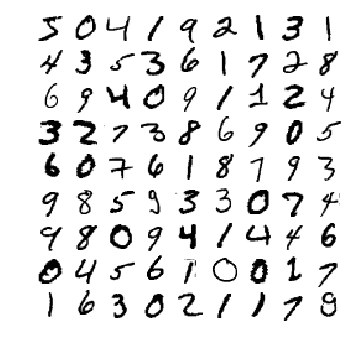
\includegraphics[width=0.4\textwidth]{images/mnist_v2}
    \caption{Przykładowe dane ze zbioru MNIST}
    \label{fig:mnist}
\end{figure}

\section{Autoenkoder wariacyjny}

Chciałbym zacząć od sprawdzenia podstawowych własności autoenkodera wariacyjnego, przedstawionych w rozdziale \ref{sec:vae} W tym celu wytrenowałem modele o różnych rozmiarach reprezentacji ukrytej: 2, 5, 7, 20, 50. Następnie sprawdziłem jak radzą sobie z rekonstrukcją danych ze zbioru testowego oraz generowaniem nowych próbek. Wyniki prezentują się na rysunku \ref{fig:mnist_recon}. 

\begin{figure}[h!]
  \centering
  \begin{subfigure}[b]{0.45\linewidth}
    \missingfigure[]{ Rekonstrukcje z podziałem na rozmiary reprezentacji }
    \caption{}
  \end{subfigure}
  \begin{subfigure}[b]{0.45\linewidth}
    \missingfigure[]{ Box plot z rozkładem błędów średniokwadratowych }
    \caption{}
  \end{subfigure}
  \begin{subfigure}[b]{0.45\linewidth}
    \missingfigure[]{ Generowanie nowych próbek }
    \caption{}
  \end{subfigure}
  \caption{}
  \label{fig:mnist_recon}
\end{figure}

Ze względu na łatwość wizualizacji, do sprawdzenia jak dane reprezentowane są w przestrzeni ukrytej wybrałem model bazujący na wymiarze rozmiaru 2. Zdaję sobie sprawę, że rekonstrukcje w tym przypadku nie są najlepszej jakości, ze względu na zbyt ograniczoną ilość informacji możliwych do przekazania, ale zależy mi też na przedstawieniu podstawowych założeń. W tym celu na wykresie dla losowych próbek zaznaczyłem odpowiadające im średnie oraz odchylenia. Otrzymany rezultat widać na obrazku \ref{fig:mnist_2d}, gdzie można zauważyć opisane wcześniej własności wybranego modelu takie jak skoncentrowanie reprezentacji wokół $\vec{0}$ czy ciągłość przestrzeni.

\begin{figure}[h!]
    \centering
    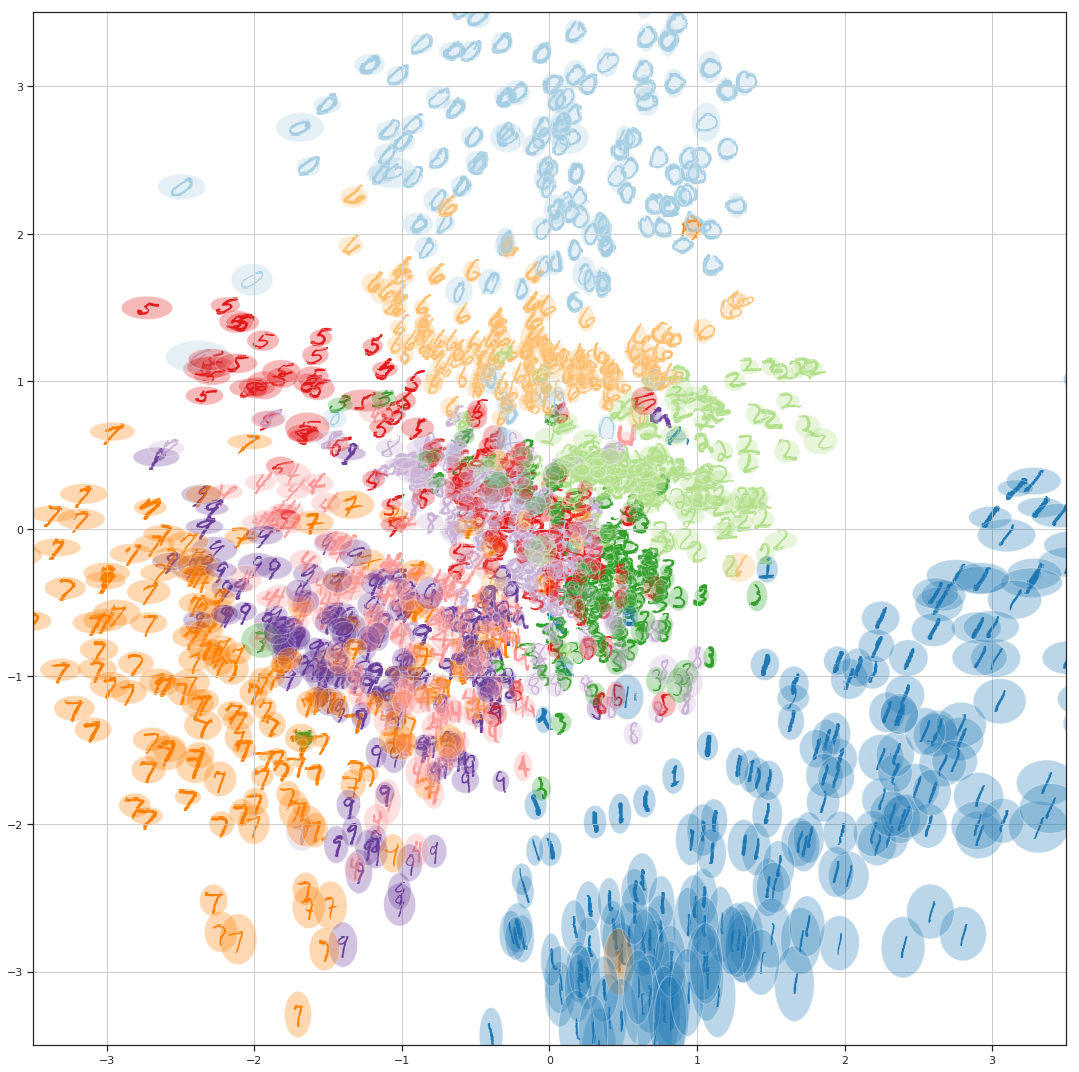
\includegraphics[width=1.\textwidth]{images/mnist_2d}
    \caption{}
    \label{fig:mnist_2d}
\end{figure}

\subsection{Symulacja docelowego problemu}

Na początek chciałbym zacząć od odtworzenia docelowego problemu na prostszych danych jakim jest zbiór MNIST. Pozwoli to w ogólności stwierdzić sensowność skorzystania z wybranego modelu. Zakładam, że jeśli eksperyment nie powiódłby się na łatwiejszych danych, to raczej nie powiedzie się również na tych bardziej skomplikowanych. To miejsce traktuje jako poligon testowy. Pozwoli mi to też nabrać pewnego rodzaju doświadczenia z wybranym modelem.

Sytuację, którą będę chciał poddać testowi jest całkowite niezbalansowanie danych, a wręcz brak danych drugiej kategorii i obserwacja jak zachowuje sie w takim przypadku model. Będę chciał to osiągnąć poprzez uczenie modelu jedynie na danych pochodzących z dwóch klas [4, 7], a następnie obserwacja tego co się stanie z modelem przy zaaplikowania danych z klasy [5]. Ma to odtworzyć sytuację gdzie danych opisujących zmiany nowotworowe jest przytłaczająco mniej od tych zdrowych.

W oryginalnym problemie mamy bardzo duży dysonans pomiędzy ilością przykładów dla każdej z klas. Według statystyk dane z komórkami rakowymi stanowią ~1\% wszystkich. Ciężko jest wiec nawet mówić o jakimś sensownym podejściu supervised. Do zasymulowania tego problemu dla MNIST będę uczył model jedynie na dwóch klasach [4, 7], a następnie testował zachowanie reprezentacji ukrytej dla przekładów z klasy 5.

Rozmiar reprezentacji ukrytej wynosi 10. Analizować natomiast będziemy 2 składowe kosztu dla modelu VAE: KLD oraz błąd rekonsrukcji MSE. Na rysunku \ref{fig:mnist_compare} znajduje się przedstawienie ich wraz z histogramami. Można zauważyć, że wyłącznie na podstawie samego błędu rekonstrukcji można z bardzo dużą dokładnością określić dane pochodzące z klasy 5, mimo iż model nie widział żadnych ich przykładów podczas uczenia.

\begin{figure}[h!]
    \centering
    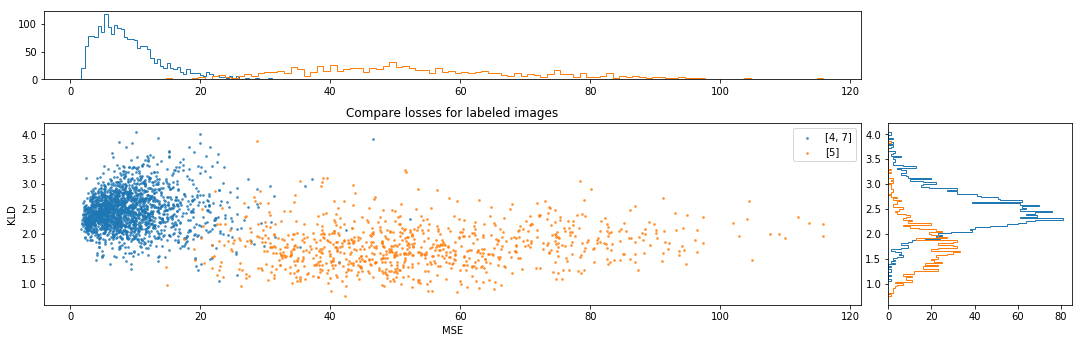
\includegraphics[width=1.0\textwidth]{images/mnist_compare}
    \caption{}
    \label{fig:mnist_compare}
\end{figure}

Do określenia jak rzeczywiście dobra jest ta separacja można wykorzystać krzywą ROC. Traktujemy to jako problem binarnej klasyfikacji, gdzie dane z klasy 5 będą oznaczone jako 1, a z [4, 7] jako 0. Wartość confidence to suma kosztów KLD i MSE. Jak widać na rysunku \ref{fig:mnist_roc} takie podejście osiąga prawie 100\% skuteczność. Podobne podejście będę chciał zastosować do danych medycznych.

\begin{figure}[h!]
    \centering
    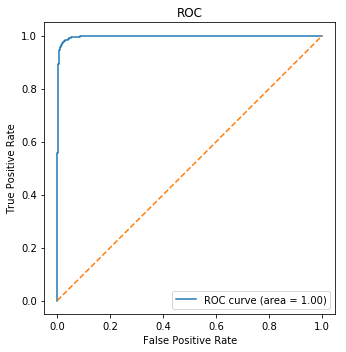
\includegraphics[width=0.5\textwidth]{images/mnist_roc}
    \caption{}
    \label{fig:mnist_roc}
\end{figure}

\section{Deep feature consistent variational auto-encoder}

Podobny eksperyment jw. przeprowadziłem również dla modelu DFC. Na początku jednak warto zobaczyć co zyskujemy na zmianie podejścia do kosztu rekonstrukcji. Różnice prezentują się na rysunku \ref{fig:vae_dfc_recon}. Widać, że rekonstrukcje są mniej rozmazane niż przy standardowym VAE. Dodatkowo lepiej rekonstruuje takie elementy jak np. pozioma kreska w cyfrze 7. 

\begin{figure}[h!]
    \centering
    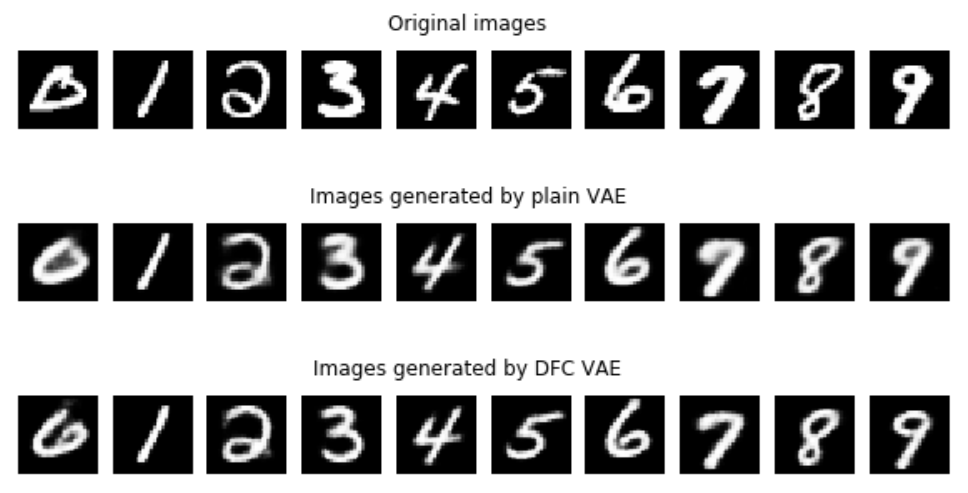
\includegraphics[width=0.8\textwidth]{images/vae_dfc_gen}
    \caption{}
    \label{fig:vae_dfc_recon}
\end{figure}

Na rysunku \ref{fig:dfc_mnist_compare} przedstawiony jest efekt przeprowadzenia analogicznego eksperymentu z nauką na jedynie przykładach z klas [4, 7] i sprawdzeniu zachowania dla danych z klasy 5. Zamiast kosztu rekonstrukcji MSE używamy błędu perceptualnego. Dodatkowy model splotowy również nie widział danych pochodzących z 5 klasy. Jak widać separacja jest co najmniej tak dobra jak w przypadku zwykłego VAE.

\begin{figure}[h!]
    \centering
    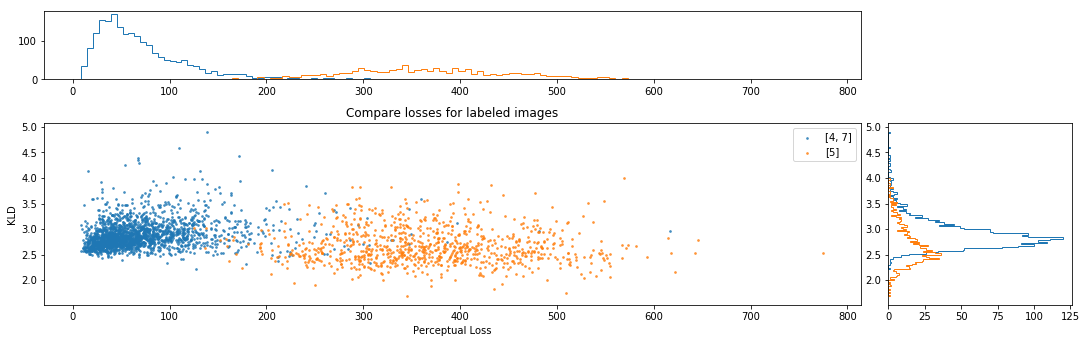
\includegraphics[width=1.0\textwidth]{images/dfc_mnist_compare}
    \caption{}
    \label{fig:dfc_mnist_compare}
\end{figure}

\section{Conclusion}

Na podstawie otrzymanych wyników mogę stwierdzić, że eksperyment się powiódł. W przypadku danych MNIST udało się sklasyfikować dane, których wcześniej nie widzieliśmy. Jest sens w takim razie w użycie tego modelu dla już prawdziwych danych.
